\chapter{Immersed Boundary Methods}
\label{CHAPTER:IBM}.

\section{Introduction}

For many fluid problems it is mandatory to solve the equations of motion with respect to complex-shaped geometries.
The algorithm introduced in chapter \ref{CHAPTER:CUDA} is not yet suitable for such a scenario.
For instance the simulation inside a spheric geometry is not possible, since the boundaries
do not coincide with the implemented cartesian grid. Nevertheless there exist different approaches to overcome this problem
which shall be introduced here. \\
One common approach to extend the algorithm it the use a body-fitted mesh.
Different advantages and disadvantages arise with this kind of implementation, see \citep{Mittal2005}.
One benefit is a much simpler deployment of the desired boundary condition, due to the overlap of the numerical grid with domain borders.
Furthermore a higher accuracy can be achieved \citep{Gornak2013}.
However, using an unstructered grid generates  computational overhead, during and before the execution of a simulation.
The grid generation algorithm can be complicated in contrast to using a cartesian grid. This can be even more difficult when
moving boundaries are considered.
Moreover, solving the finite differenc schemes on a curvilinear coordinate system, requires more calculations for a single grid point.
The last important aspect is the implementation on the GPU.
Like discussed in section \ref{cuda:sec_performance} it is more efficient to use homogeneous storage and calculation pattern on a CUDA-device,
the use of unstructured data makes this very difficult.

A set of alternative methods, to resolve the problems described above, are so called Immersed Boundary Methods.
The term was first mentioned in \citep{peskin72}, where the method was used for the simulation of blood flow through a heart valve,
but has since then been used for a variety of methods \citep{Mittal2005}.
All of them have the idea in common to perform the simulations on a cartesian grid which does not conform to the domain boundary.
To satisfy the desired boundary conditions additional terms are introduced into the equations of motion.
In general one can distinguish between continuous forcing methods and direct forcing methods.
Continuous forcing methods try to mimic the boundary using a localized forcing term which acts on all points near to the boundary.
Since the surface is often described by lagrangian points, these methods are well suited for moving boundaries \citep{Mittal2005}.
Direct forcing approaches try to satisfies the boundary conditions by imposing them directly to points at the fluid boundaries for often with the use of an interpolation procedures.
Some of the major drawbacks using Immersed Boundary methods is the loss in  spatial accuracy at the boundary due to interpolation or approximations. Therefore it can be necessary to use a higher grid resolution
compared to a body-fitted mesh.
The benefits of these methods is the use of a cartesian grid, which is much more suited for a GPU-based implementation, see Sec. \ref{cuda:sec_threadmanage}.
One objective of this chapter is to introduce implementation of NoSlip boundaries for cartesian grids, with the use of Immersed Boundary methods.
The term Immersed Boundary Method is vaguely defined in literature, in this thesis we refer with it to all methods introduced in this chapter..

\section{Immersed Boundary Methods}

For the purpose of discussion the different methods introduced here will be applied to a default geometry.
The fluid domain without any immersed boundaries is set to a cube of the size $l_i= 1$ with  $i \in \{x, y, z\}$.
For the discretization we choose $N_i = 32$ for the number of grid points.
As an example of an immersed boundary, we will discuss the embedding of a cylinder, given by the  surface equation

\begin{align}
    \label{ibm:eq_cylinder_intro}
    \left(x - \frac{l_x}{2}\right)^2 + \left(y - \frac{l_y}{2}\right)^2 = r^2
\end{align}

where $r=0.4$ is the radius and the center is given by $(l_x/2, l_y/2)$.
The simulation domain is than separated into the fluid domain $\Omega_f$ and the wall domain $\Omega_w$.
The overall goal is to enforce the No-Slip condition $\vec{v} = 0$ on the surface $\partial \Omega_f$, furthermore
the conservation of mass should be fulfilled.


\subsection{Volume Penalization}
\label{chap:ibm_volpen}
The concept behind the volume penalization method is to introduce an additional forcing term into the Navier-Stokes equation, which acts on
the grid points outside of the fluid domain to ensure the desired boundary conditions. The methods was successfully implemented and tested
on pseudo-spectral methods, see for example \citep{Lulff2011}.
For the implementation it is necessary to define a masking function $H(x, y, z)$ which seperates the simulation domain into $\Omega_f$ and $\Omega_w$.
For a cylinder the surface equation \label{ibm:eq_cylinder_intro} can be modified to
\begin{align}
    \label{ibm:masking_function}
H(x, y, z) = \begin{cases}
                    0, &  \left(x - \frac{l_x}{2}\right)^2 + \left(y - \frac{l_y}{2}\right)^2 <r^2\\
                    1, & \text{else}
             \end{cases}
\end{align}

With this function an additional forcing term can be added into the Navier-Stokes equation

\begin{align}
    \label{ibm:vp_navstok}
    \pdn[u]{t} + \vec{u} \cdot \vec{\nabla} \vec{u} &= -c^2 \nabla \rho + \frac{1}{Re} \Delta \vec{u} + \vec{F}_{ext}
     +\underbrace{ \frac{H(x, y, z)}{\nu}(\vec{v} - \vec{v_0})}_{\text{Vol. Pen. Forcing}}
\end{align}

where $\nu$ is a regulation parameter also denoted as damping rate of the forcing and $\vec{v}_0$ is the desired Dirichlet boundary condition.
Hence, for No-Slip boundaries it is $\vec{v}_0 = 0 $.
The additional term in Eq. \ref{ibm:vp_navstok} acts as an exponential damping force on a single grid point.
The forcing acts inside of $\Omega_w$ as $H(x, y, z) = 1$ and vanishes in $\Omega_f$.
The strength of the forcing is scaled by the damping rate $\nu$.
For a small $\nu$ a stronger forcing is applied to the points in $\Omega_w$.
It can be shown that for $\nu\rightarrow 0$ the velocity in $\Omega_w$ converges against zero
and the No-Slip boundaries are fulfilled \citep{Lulff2011}.
However, the additional term in Eq. \ref{ibm:vp_navstok}
also introduces an additional stability criterion \citep{Lulff2011}, that is

\begin{align}
    \label{ibm:eq_vpcrit}
    \Delta t < \Delta t_{VP} := \nu
\end{align}

The time step is already severely restricted due to the method of artificial compressibility, see Sec. \ref{num:sec_articomp}
Hence, the criterion given by Eq. \ref{ibm:eq_vpcrit} is not of concern.
The implementation of the Volume-Penalization method is rather simple.
The masking function is defined before runtime.
During runtime for each grid point ${(i, j, k)}$ the value ${H(i\Delta x, j\Delta y, k \Delta z)}$,
is stored into an additional array located on the global memory of the GPU.
This value is than loaded during the computation of a time step.
For the cylinder this masking array is show in Fig. \ref{fig:ibm_maskvolpen}.
It can be noted that the major-drawback of this method is a pixelated border.
The exact boundary can only be satisfied for $\Delta x$, $\Delta y$ and $\Delta z \rightarrow 0$.

\begin{figure}[!t]
    \centering
    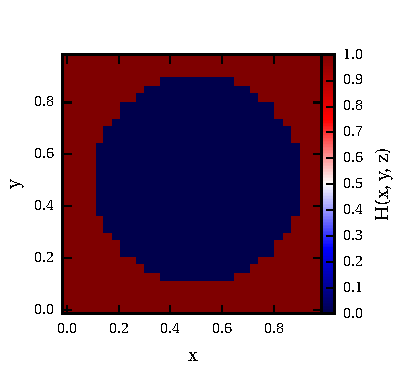
\includegraphics{gfx/immersed_boundary/methods/mask_volpen.pdf}
    \caption{Masking array $H(i,j,k=const.)$ for a cylinder, in the (x,y) plane.}
    \label{fig:ibm_maskvolpen}
\end{figure}

\subsection{Direct Forcing}
\label{chap:ibm_dirforce}

One concern of the Volume-Penalization method is the remaining velocity in the wall domain close to the boundaries.
The Direct-Forcing method bypasses this restriction by an implicit calculation of the forcing term.
This method was first mentioned by \citep{mohdyusof:1997} and is discussed in detail in \citep{Fadlun2000}.
With the use of the Euler method the discretization of the Navier-Stokes Equation can be written as

\begin{align}
    \label{ibm_df_method_lame}
    \frac{\vec{u}^{n+1} -\vec{u}^n}{\Delta t} = \mathscr{L}^* + \vec{f}\\
\end{align}

where $\mathscr{L^*}$ are the discretized advection and viscous terms and the density gradient and $\vec{f}$ is the forcing term.
For a boundary point the condition $\vec{u}^{n+1} = \vec{u}_0$ should hold.
By substituting this expression into Eq. \ref{ibm_df_method_lame} it follows that
\begin{align}
    \frac{\vec{u}_0 -\vec{u}^n}{\Delta t} = \mathscr{L} + \vec{f} \Rightarrow \vec{f} = \frac{\vec{u}_0 -\vec{u}^n}{\Delta t\cdot \mathscr{L}}\\
\end{align}

The implementation of this method is similar to the Volume-Penalization method.
A masking array is computed before the execution of a simulation.
The forcing term is than added into the register $Q_\Phi$ (see Sec. \ref{sec:cuda_timestep}) after the computation of $\mathscr{L}$.
It can be noted that this procedure is equivalent to simply setting $\vec{v}=0$ after a time step.
However this is not the possible when the boundaries are further improved for example with the Volume-Fraction method.
For now the major-drawback of the Direct-Forcing method is a pixelated border.
In contrast to the Volume-Penalization method no further stability criteria are introduced.

\subsection{Volume Fraction Interpolation}

The methods introduced so far lack the ability of an exact implementation of the boundary conditions on $\Omega_f$.
Instead the surface $\partial \Omega_f$ is described by the nearest grid points in $\Omega_w$, resulting in a
stepwise approximation.
To overcome this problem a simple procedure is the use of an volume fraction interpolation scheme, introduced in \citep{Fadlun2000}.\\
The advantage of this method is the simple implementation into the volume penalization and direct forcing method.
Furthermore the overall computation time of the time step stays constant, in  contrast to complex interpolation schemes.\\
Initially the interpolation begins by determine all grid cells which are cut by the surface $\partial \Omega_f$.
For each of these boundary cells the total volume $V_w$ of the wall domain $\Omega_w$ inside each cell is computed.
This method can be applied to the Volume-Penalization and the Direct-Forcing method.
The force acting on the points inside the boundary cells is than weighted by a scaling factor, $\Phi = V_W/(\Delta x \Delta y \Delta z)$.

\begin{figure}[!bp]
    \centering
    \subfloat[Masking array H(i, j, k=const.) for the Volume-Fraction method]{{
      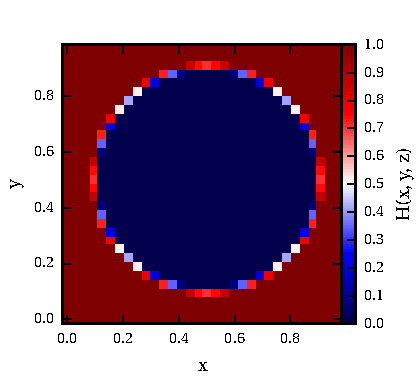
\includegraphics{gfx/immersed_boundary/methods/mask_volfrac.pdf}\label{fig:mask_volfrac}
      \label{ibm_volfrac_masking_array}
        }}%
    \qquad
    \subfloat[Convergence of the relative $l_2$-error of the Monte Carlo integration]{{
      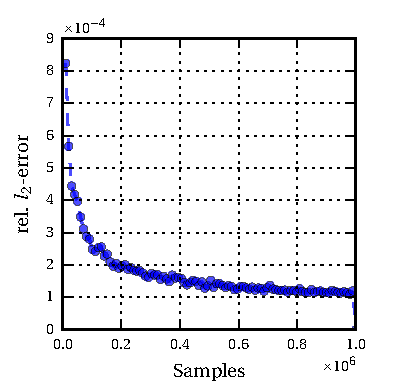
\includegraphics{gfx/immersed_boundary/methods/error_volfrac.pdf}\label{fig:error_volfrac}
        }}%
      \label{ibm_volfrac_montecarlo}
    \label{fig:example}%
\end{figure}

For the implementation an improved version of the masking array $H$ is used.
Like in the previous methods the masking array is precomputed and loaded at runtime. The algorithm is extended to compute the
volume fractions of the cells lying next to the surface $\partial\Omega_f$.
Since an exact computation is difficult to implement for arbitrary surfaces one option is to use a Monte Carlo integration method.
For each cell $N$ random samples are generated, then the volume fraction is simply given by the ratio of samples lying in- and outside outside the fluid domain.
This is determined by using the masking function $H(x, y, z)$.

An example for the generated masking array with $N=2e5$, is shown in Fig. \ref{ibm_volfrac_masking_array}.
The symmetric distribution of the boundary values indicates
a good approximation. For a better evaluation a convergence study was performed were the number of samples $S$ was varied between 100 and $10^6$ points.
The $l_2$-error was determined by comparing the results to the computation with the highest number of samples.
The results are shown in figure \label{ibm_volfrac_montecarlo}.

For the number of samples in the interval below $S=2\dot10^5$  a fast decay in the error to the order $2\dot10^{-4}$ can be observed.
Above this interval the error is of the order $10^{-4}$.
It can be concluded that the integration should be accurate enough by using $S=10^5$ samples.

\clearpage
\subsection{Interpolation Method}

The last immersed boundary method introduced in this thesis is a bilinear interpolation method, which was first presented by \citep{Gilmanov2003}.
One difference to the previous methods is an exact representation of the immersed boundary, instead of a pixelated one.
A schematic representation of the interpolation procedure is shown in Fig. \ref{ibm:ip_method_algo}.

\begin{figure}[!bp]
      \centering
        \resizebox{0.8\textwidth}{!}{
       \import{gfx/immersed_boundary/methods///}{ip.pdf_tex}
      }
      \caption{Interpolation of the velocity of the point $b$. The point $c$ is a projection from the point $a$ into the direction of the normal $\vec{n}$,
       onto the plane defined by the grid points $\alpha$, $\beta$, $\gamma$ and $\delta$. The immersed boundary is given by the masking function H(x,y,z).
       For the bilinear interpolation the coefficient $c_1$ and $c_2$ are used.
      }
    \label{ibm:ip_method_algo}
\end{figure}

The interpolation method is applied to all grid points which posess a nearest neighbor outside of the fluid domain.
In this setup this is true for the point $b$, for which the velocity $\vec{v}$, shall be interpolated.
The idea of this method is to linear interpolate $b$ into the direction of the normal $\vec{n}$, of the immersed boundary.
The intersection of the interpolation direction with the boundary is given by the point $a$, with the distance $\Delta h =[ab]$.
The point $b$ is  projected into the direction of the normal $\vec{n}$, onto the plane defined by
the nearest grid points $\alpha$, $\beta$, $\gamma$ and $\delta$.
After the position calculation of the point $c$, the velocitiy $\vec{v}(c)$ is obtained by a bilinear interpolation
of the velocities at the points $\alpha$, $\beta$, $\gamma$ and $\delta$, given by (\citep{numrecipes})

\begin{align}
    \vec{v}(c) =  \frac{1}{\Delta x\Delta y} \left(\vec{v}(\beta)(\Delta x -  c_1)(\Delta y -  c_2) +
            \vec{v}(\gamma)(\Delta x -  c_1)(c_2) +
            \vec{v}(\alpha)(  c_1)(\Delta y -  c_2) +
            \vec{v}(\delta)( c_1)(c_2) \right)
\end{align}

where $(c_1, c_2)$ is the offset from $c$ to $\beta$, or in general the offset to the point of the plane, which is closest to $b$.

With the obtained velocity $v(c)$ and  the No-Slip boundarie condition $v(a) = 0$,
the interpolated velocity is given by
\begin{align}
    \vec{v}(b)  =  \vec{v}(c)\frac{\Delta c}{\Delta h}
\end{align}
where $\Delta c = [ac]$.

For a simplification of the interpolation procedure for different geometries, a preprocessing routine was implemented.
In order to interpolate a certain geometry three functions have to defined.
A masking function $H(x, y, z)$, a function which gives the distance to the boundary $d(x, y, z)$
and a function $\vec{g}(x, y, z)$ with determines the normal direction  of the boundary.
For the cylinder the masking function $H(x, y, z)$ is given by Eq. \ref{ibm:masking_function}.
The distance is

\begin{align}
    d(x, y, z) = \sqrt{\left(x - \frac{l_x}{2}\right)^2 + \left(y - \frac{l_y}{2}\right)^2  - r^2}
\end{align}

and the normal direction
\begin{align}
    \vec{g}(x, y, z) = \left(-\left(x - \frac{l_x}{2}\right),  - \left(y - \frac{l_y}{2}\right), 0\right)^T
\end{align}

A normalization of $\vec{g}(x, y, z)$ is performed in the algorithm,
however it is required that the normal  vectors point into the direction of the fluid domain.
Before the execution of a simulation the following steps are precomputed

\begin{enumerate}
    \item The closest point to $b$, in the example  $\beta$ is determined by the direction where $\vec{n}$ is the largest, in this example
          the $z$-direction with $n_0 := \max(\vec{n}) = n_z$.

    \item The points $\alpha$, $\gamma$, $\delta$ are determined by the remaining components ${n_y, n_z}$, which are used as directions to
            compute the offset from $\beta$.

    \item The offset $p00$, $p01$, $p10$, $p11$ of the points $\beta$, $\alpha$, $\gamma$, $\delta$ to the point $b$ are computed

    \item $\vec{n}$ is normalized by $\vec{n}^* = \frac{\vec{n}}{|n_0|}\cdot \Delta z$.
            \footnote{For $n_0=n_z$ this is $\Delta x$ and for $n_0=n_y$ it is $\Delta y$}

    \item The point $c$ is given by $c = a + \vec{n}^*$ and the coefficient $c_1$ and $c_2$ are computed and normalized to the values
           $c01 := \frac{c_1}{\Delta x}$ and $\c10 := \frac{c_1}{\Delta y}$.
    \item The ratio $W=\frac{\Delta c}{\Delta h} = \frac{d(x, y, z)}{d(x, y, z) + |\vec{n}| }$ is computed
\end{enumerate}

The values obtained from this precomputation are the offsets  $p00$, $p01$, $p10$, $p11$, the coefficients $c01$, $c10$ and
the ratio $W$. Each values is stored into an array of shape $N_x \cdot N_y \cdot N_z$, which is loaded during the simulation.
All values in the coefficient arrays which are not close to the immersed boundarie are set to zero.
During the interpolation procedure the ratio $W$ is checked and if larger than zero an interpolation for the grid point is computed.
An example of the interpolation procedure is given by

\begin{Verbatim} [fontsize=\footnotesize]
    if ((distance != 0 )){
      //load points of the plane (alpha, beta, gamma, delta)
      p00 = p00_d[global_Point] + global_Point;
      p01 = p01_d[global_Point] + global_Point;
      p10 = p10_d[global_Point] + global_Point;
      p11 = p11_d[global_Point] + global_Point;
      //load coefficients
      c01 = c01_d[global_Point];
      c10 = c10_d[global_Point];

      if (threadIdx.z == 1){
        //load velocities
        f00 = vx_d[p00]; f01 = vx_d[p01]; f10 = vx_d[p10]; f11 = vx_d[p11];
        //bilinear and linear interpolation
        f = W*(f00*(1 - c10)*(1 - c01) + f10*c10*(1 - c01)
                             + f01*c01*(1 - c10) + f11*c01*c10);
        //set the interpolated value
        vx_d[global_Point] = f;
      }
      if (threadIdx.z == 2){
        f00 = vy_d[p00]; f01 = vy_d[p01]; f10 = vy_d[p10]; f11 = vy_d[p11];
        f = W*(f00*(1 - c10)*(1 - c01) + f10*c10*(1 - c01)
                                + f01*c01*(1 - c10) + f11*c01*c10);
        vy_d[global_Point] = f;
      }
      if (threadIdx.z == 3){
        f00 = vz_d[p00]; f01 = vz_d[p01]; f10 = vz_d[p10]; f11 = vz_d[p11];
        f = W*(f00*(1 - c10)*(1 - c01) + f10*c10*(1 - c01)
                             + f01*c01*(1 - c10) + f11*c01*c10);
        vz_d[global_Point] = f;
      }
\end{Verbatim}

where \texttt{global\_Point} is the position of the interpolated point.

